The next section presents an Alloy Model for CLup. Just as a remainder, the model has been developed with the following objectives in mind: \newline

\begin{itemize}
    \item Clarity
    \item Focus on primary relevance aspects
    \item Conciseness
\end{itemize}

Subsequently, a trade-off between completeness and comprehensibility was necessary to render the model either easy at first-glance and unambiguous. \newline 
This also means some less relevant factors may have been left uncovered whereas some other pretty much basic (or predefined) elements, such as time-related ones, may have been rewritten and expanded. \newline 


{\color{gray}
\fbox{%
    \parbox {\textwidth}{%
        \small
        You may find comments along the way whenever needed. This particularly helps in achieving the clarity goal of the section while preserving conciseness and preventing the need to model elements out of the scope of this Document.

    }%
}}



\subsection{Alloy code \label{alloy_code}}


\lstinputlisting[language=alloy]{../Alloy/alloy_model_2.0.als}

\lstinputlisting[language=alloy]{../Alloy/alloy_model_2.0.als}

\begin{figure} [H]
	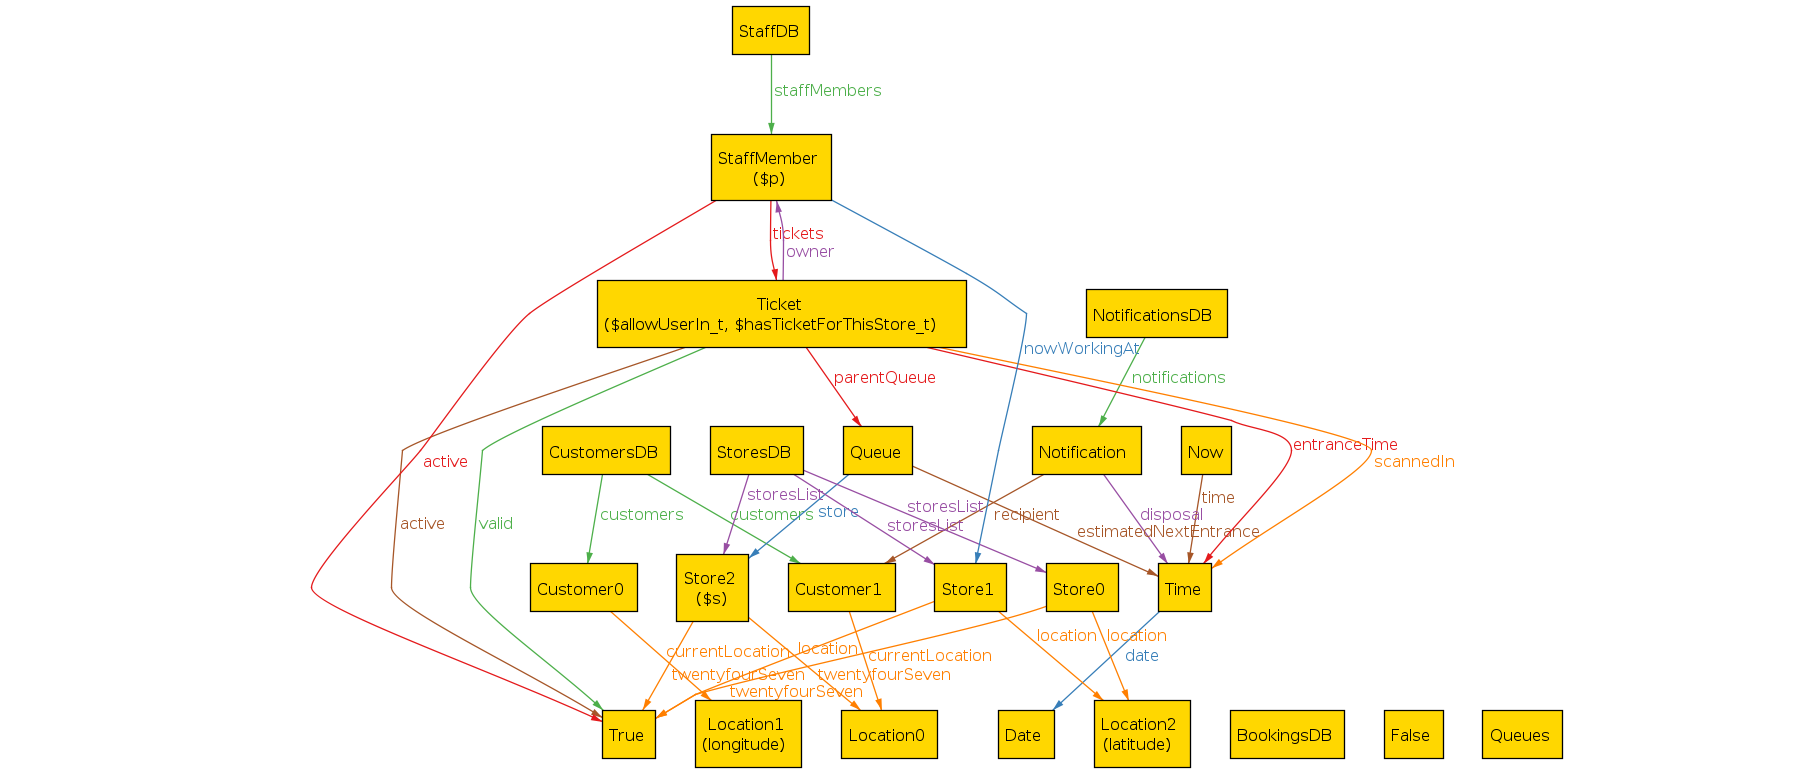
\includegraphics[width=\linewidth]{../Alloy/allowedInStaff.png}
	\caption{Descrizione diagramma alloy}
	\label{fig:AlloyTag1}
\end{figure}

\begin{figure} [H]
	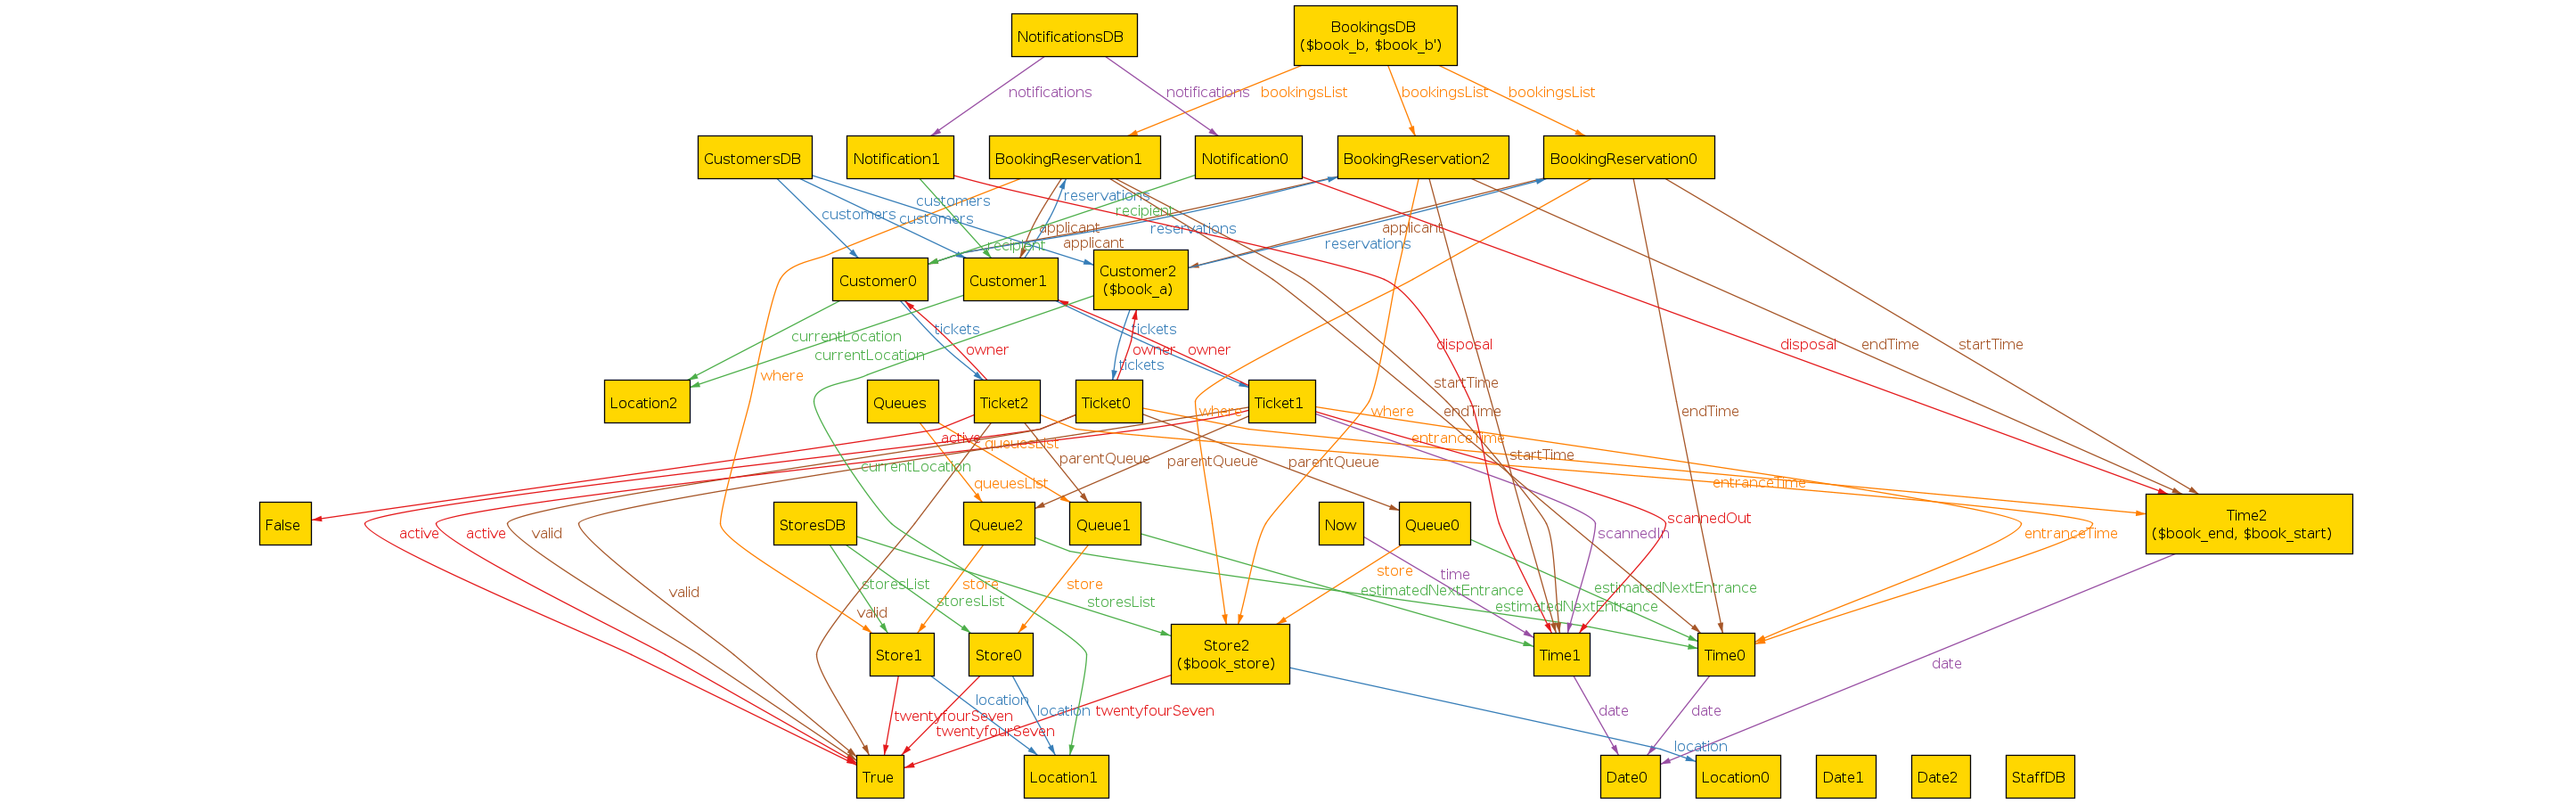
\includegraphics[width=\linewidth]{../Alloy/book.png}
	\caption{Descrizione diagramma alloy}
	\label{fig:AlloyTag2}
\end{figure}

\begin{figure} [H]
	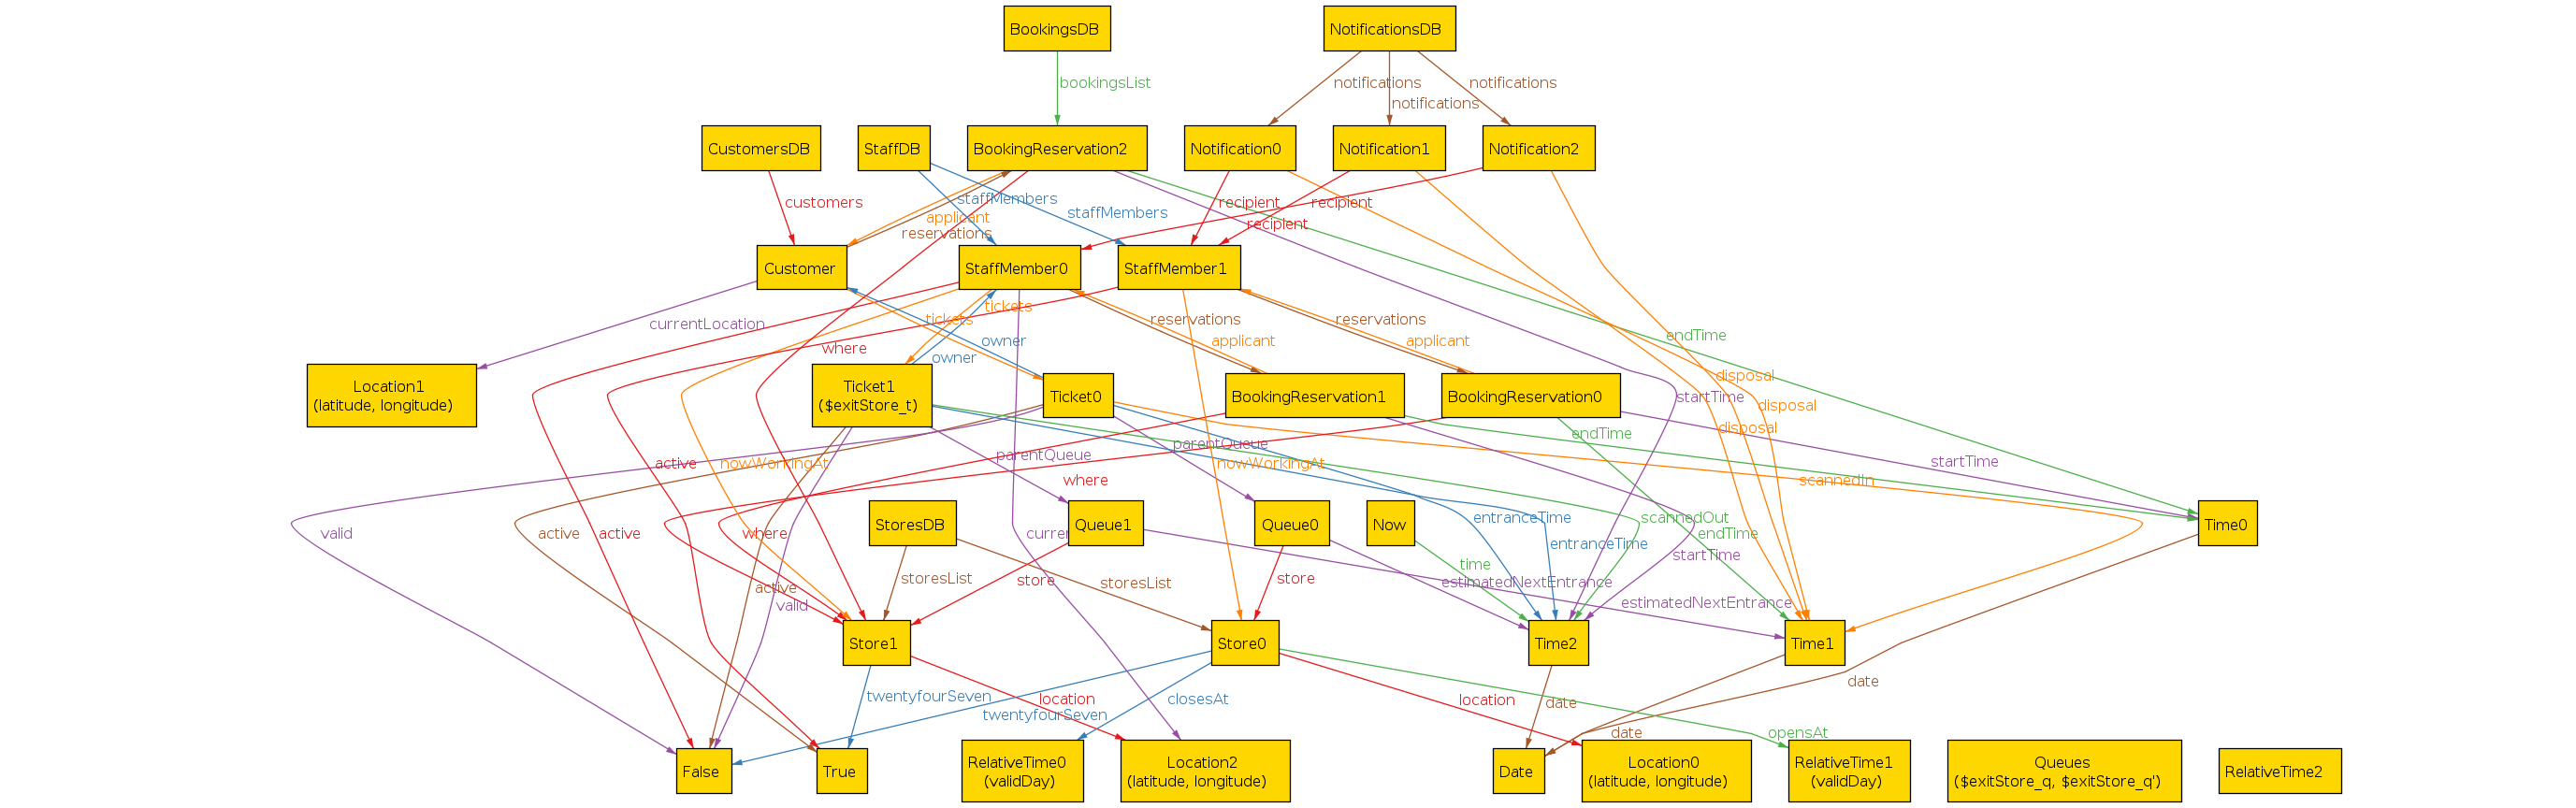
\includegraphics[width=\linewidth]{../Alloy/exitStore.png}
	\caption{Descrizione diagramma alloy}
	\label{fig:AlloyTag3}
\end{figure}

\begin{figure} [H]
	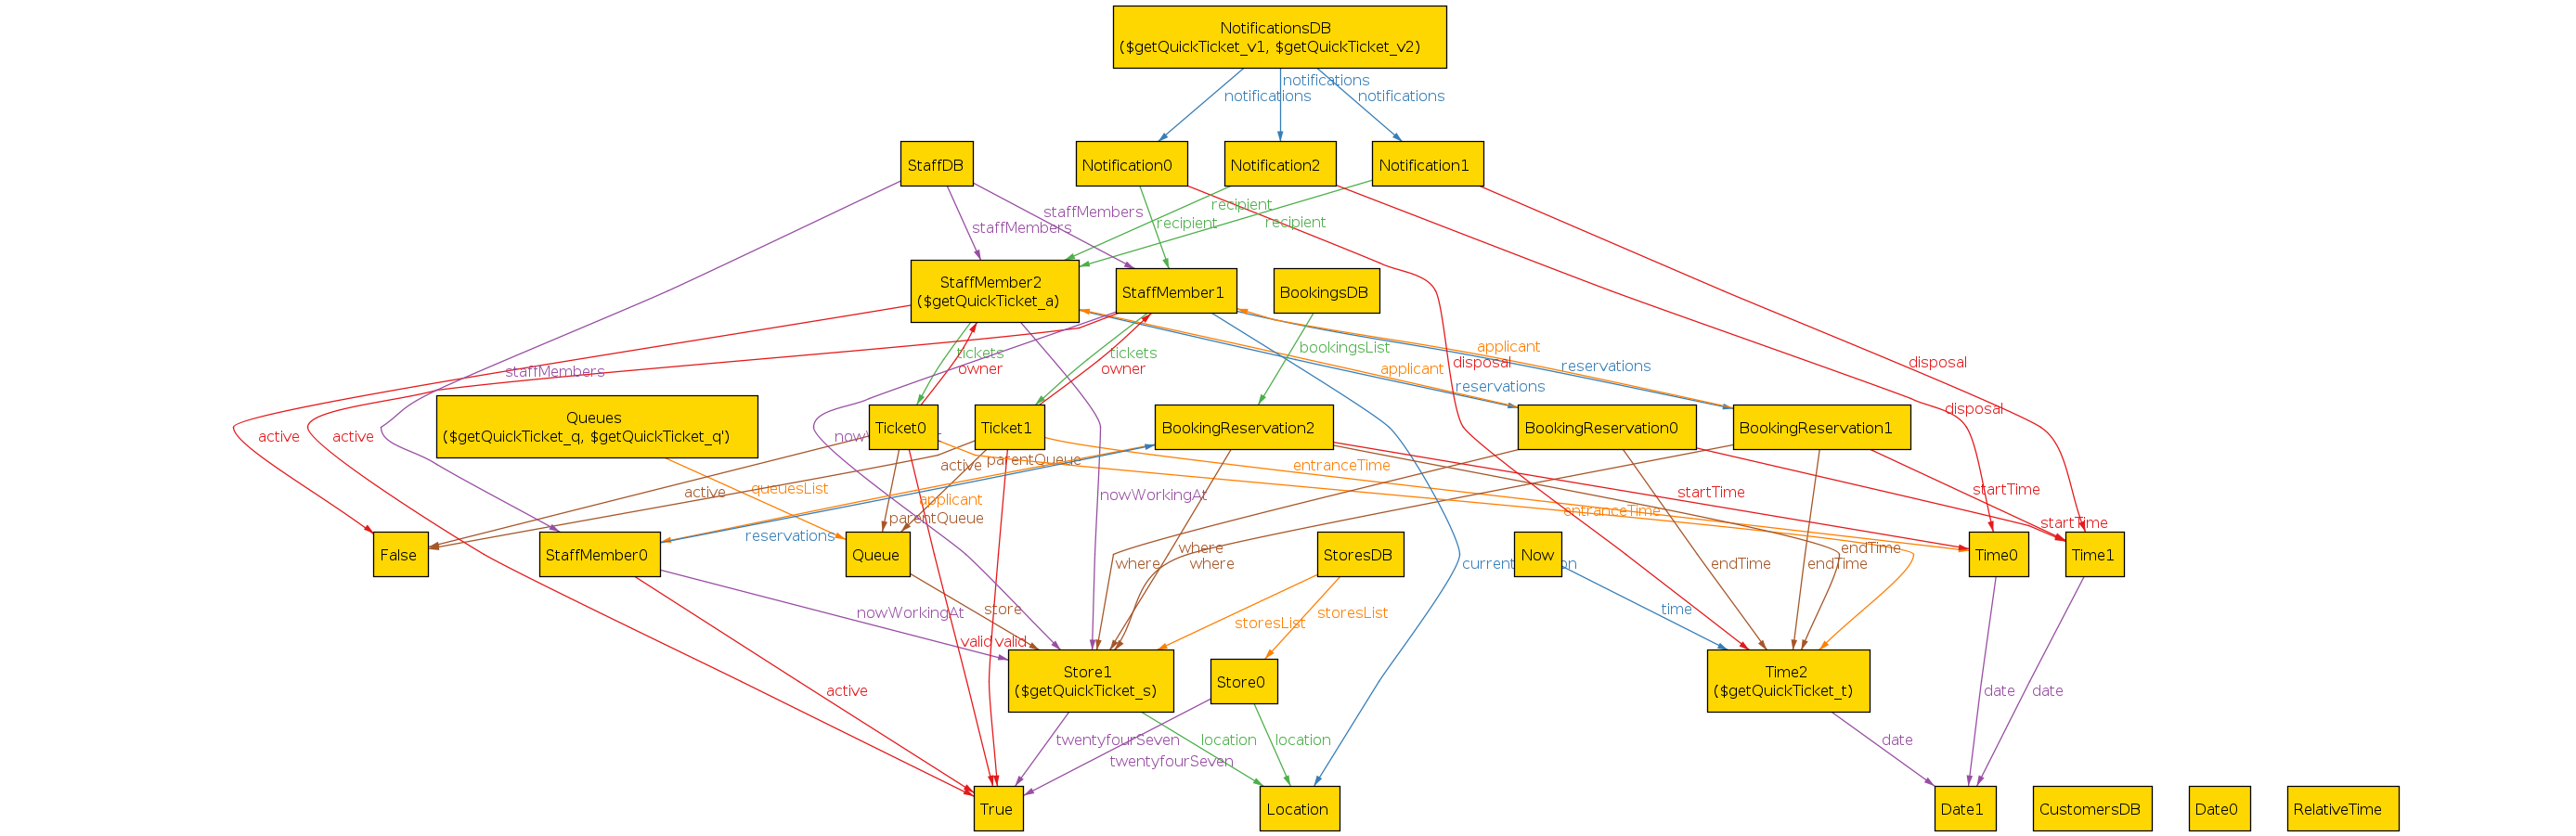
\includegraphics[width=\linewidth]{../Alloy/getQuickTicket.png}
	\caption{Descrizione diagramma alloy}
	\label{fig:AlloyTag4}
\end{figure}

\begin{figure} [H]
	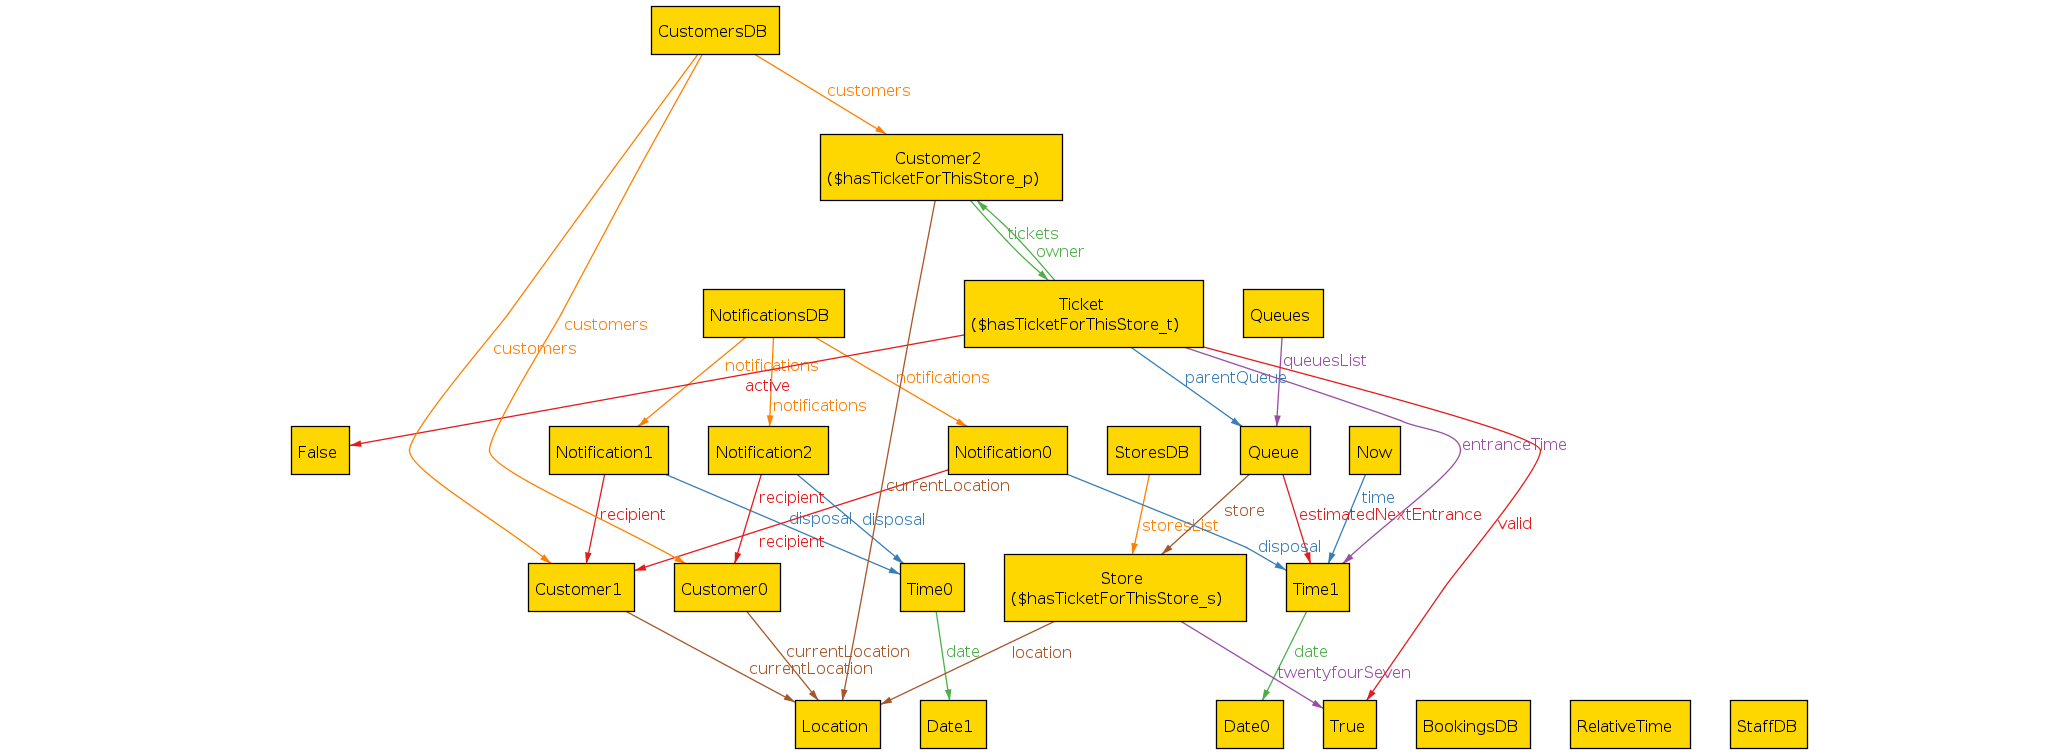
\includegraphics[width=\linewidth]{../Alloy/hasTicketForThisStore.png}
	\caption{Descrizione diagramma alloy}
	\label{fig:AlloyTag5}
\end{figure}

\begin{figure} [H]
	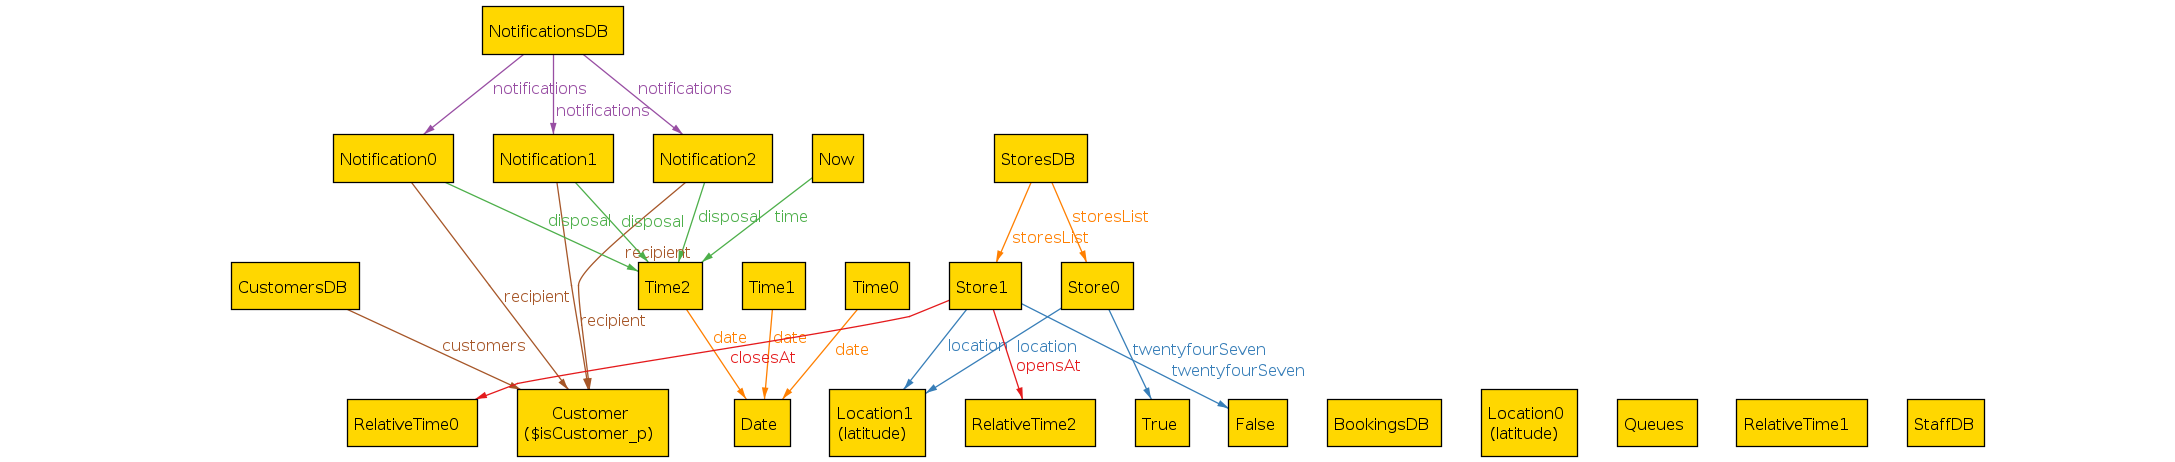
\includegraphics[width=\linewidth]{../Alloy/isCustomer.png}
	\caption{Descrizione diagramma alloy}
	\label{fig:AlloyTag6}
\end{figure}

\begin{figure} [H]
	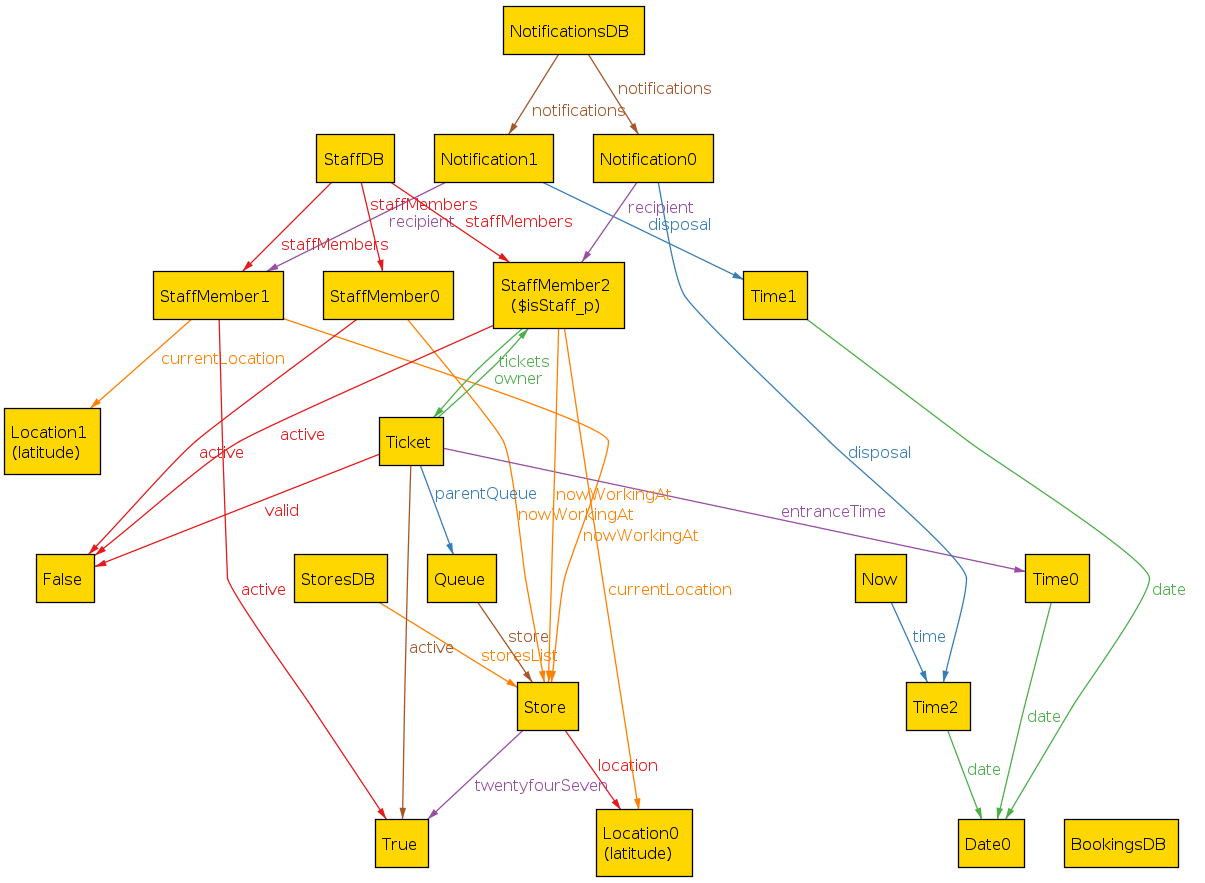
\includegraphics[width=\linewidth]{../Alloy/isStaff.png}
	\caption{Descrizione diagramma alloy}
	\label{fig:AlloyTag7}
\end{figure}

\begin{figure} [H]
	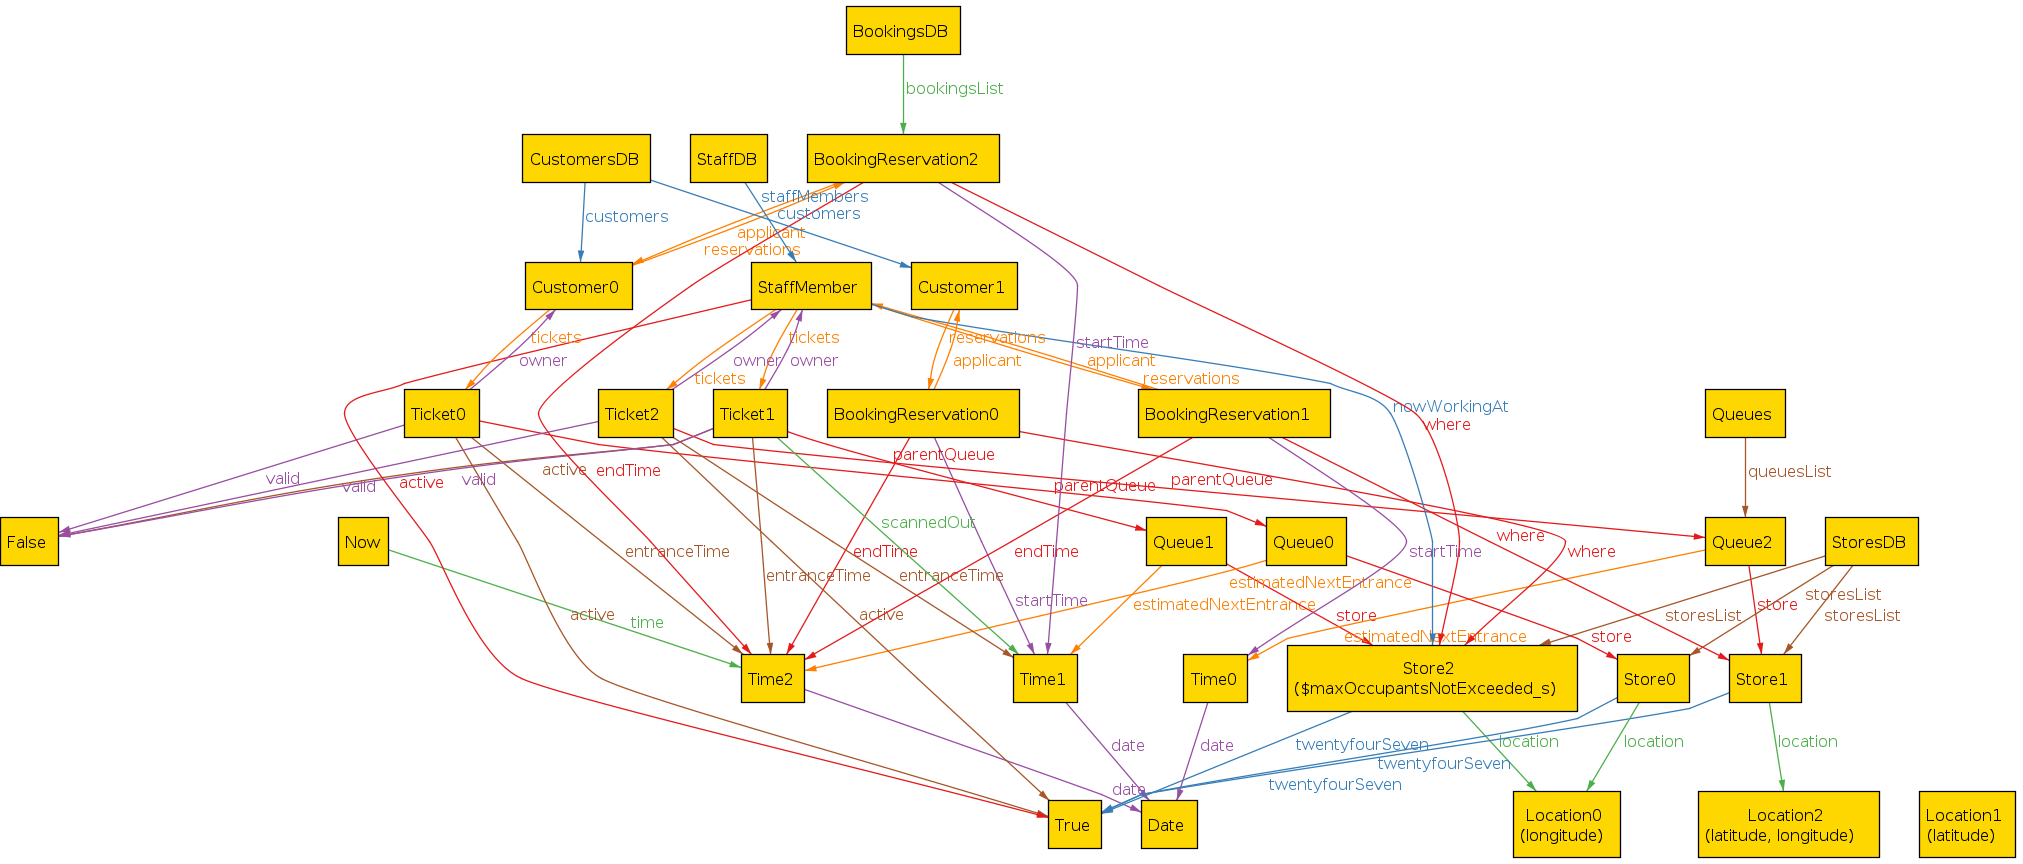
\includegraphics[width=\linewidth]{../Alloy/maxOccupantsNotExceeded.png}
	\caption{Descrizione diagramma alloy}
	\label{fig:AlloyTag8}
\end{figure}

\begin{figure} [H]
	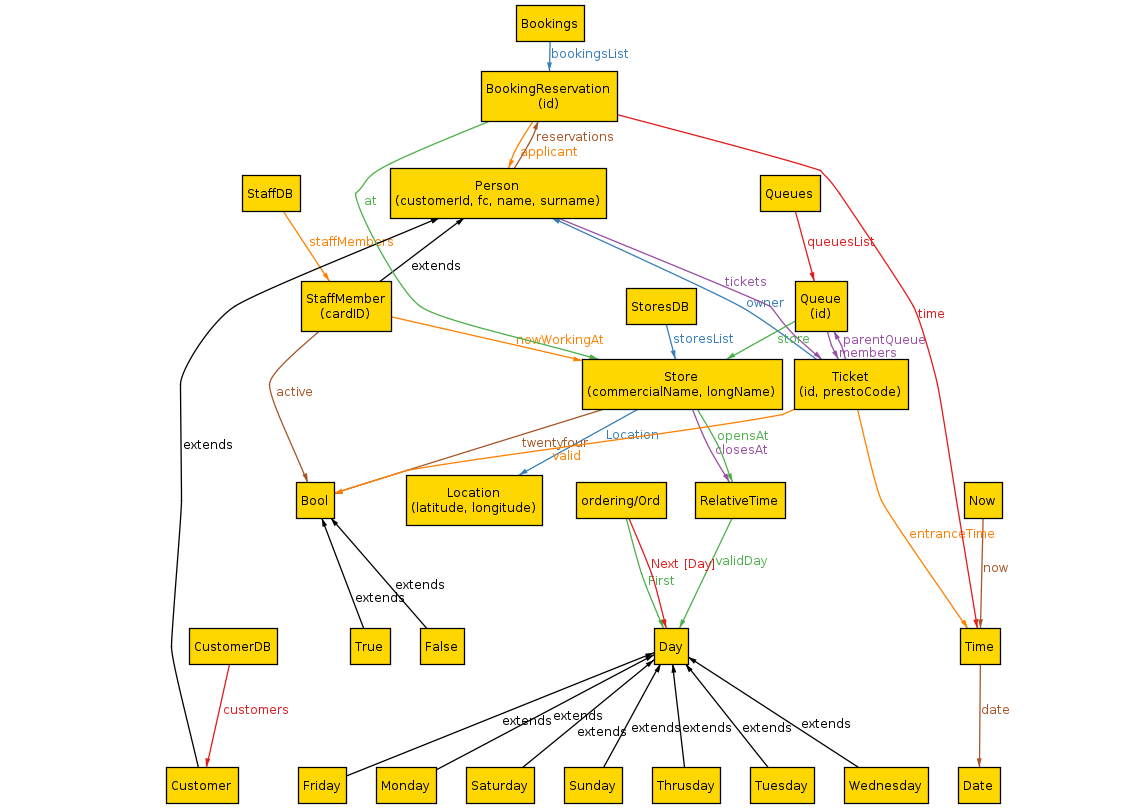
\includegraphics[width=\linewidth]{../Alloy/metamodel.png}
	\caption{Descrizione diagramma alloy}
	\label{fig:AlloyTag9}
\end{figure}

\begin{figure} [H]
	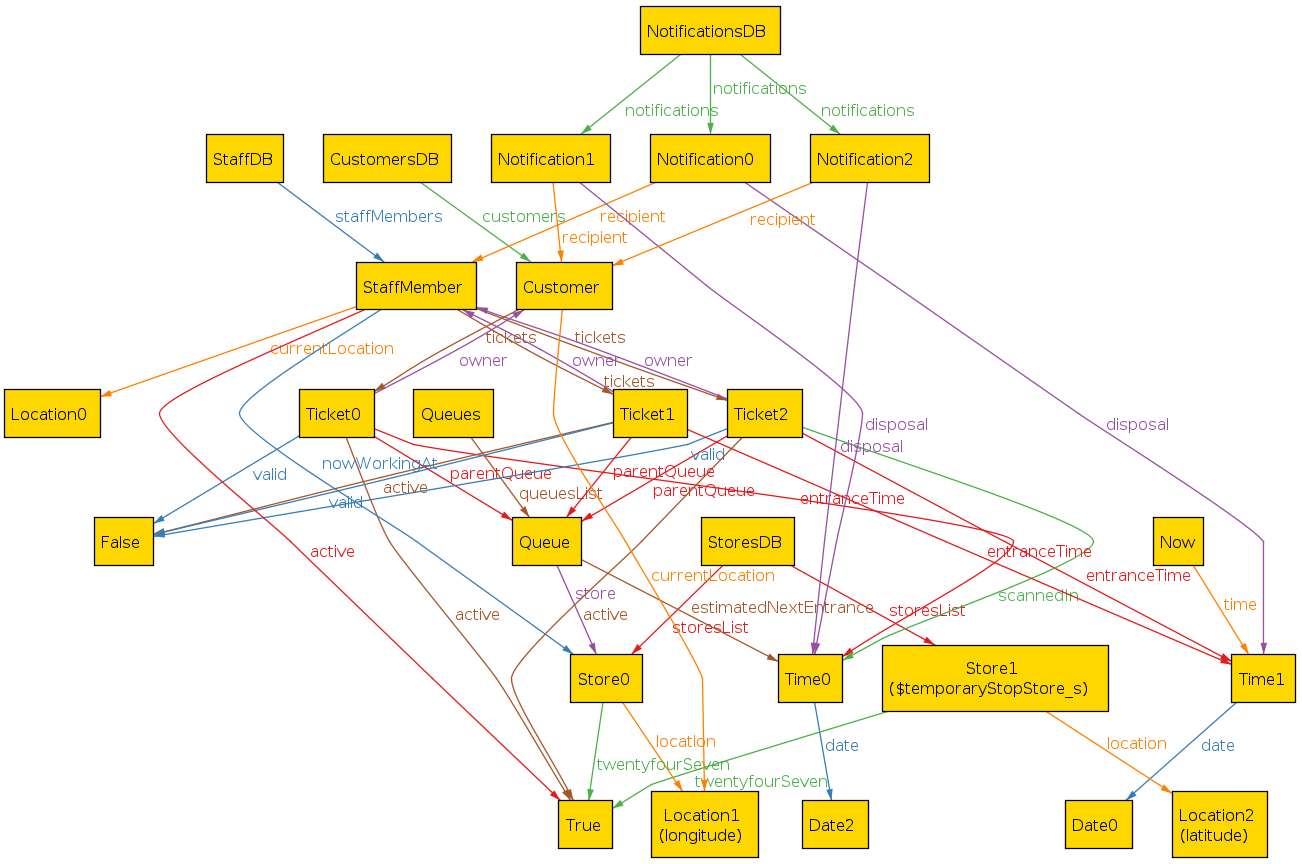
\includegraphics[width=\linewidth]{../Alloy/temporaryStopStore.png}
	\caption{Descrizione diagramma alloy}
	\label{fig:AlloyTag10}
\end{figure}

\begin{figure} [H]
	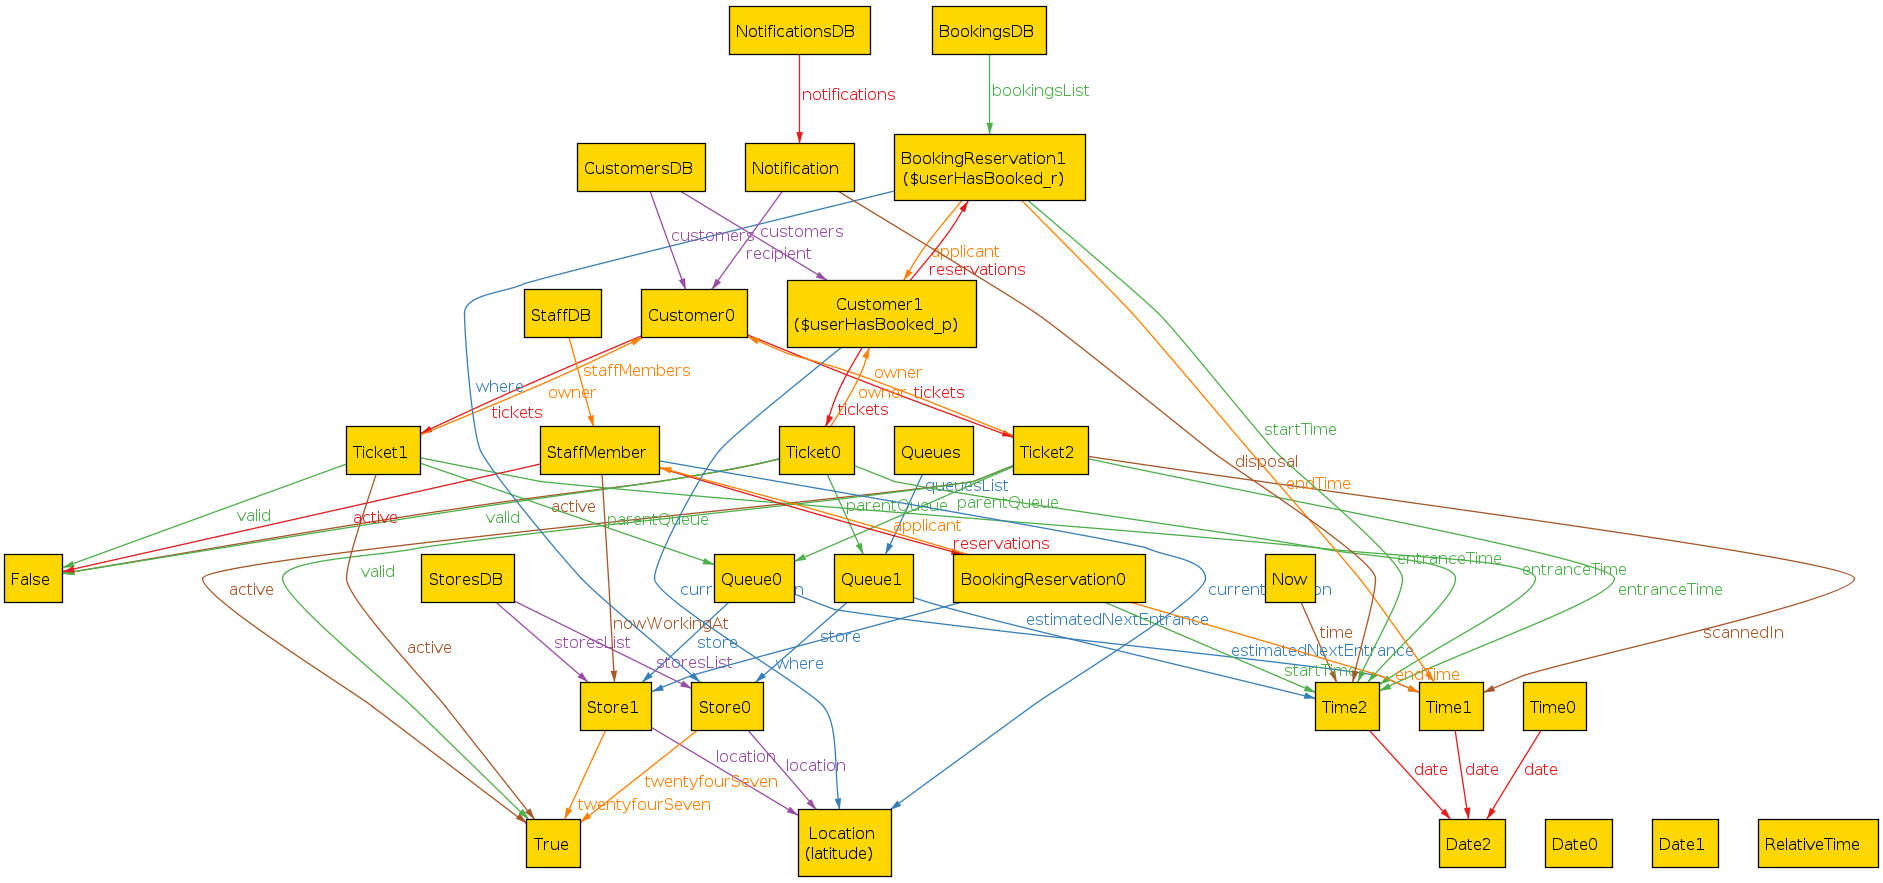
\includegraphics[width=\linewidth]{../Alloy/userHasBooked.png}
	\caption{Descrizione diagramma alloy}
	\label{fig:AlloyTag11}
\end{figure}

